\SetTitle{31}{The Quantum Fourier Transform}{Phase estimation in reverse}{31}

\begin{frame}{Overview}{What will we study?}

\begin{itemize}
    \item The \href{https://en.wikipedia.org/wiki/Fourier_transform}{Fourier Transform} is well known in physics and mathematics for its ability to represent a time-based signal as a summation of frequencies that approximates or yields the original signal.
    \item We will review the basics of the classical Fourier transform.
    \item We will study the Quantum Fourier Transform (QFT), but it turns out that this circuit is simply the \href{https://en.wikipedia.org/wiki/Quantum_phase_estimation_algorithm}{Phase Estimation} circuit, executed in reverse.
    \item The QFT is at the center of important quantum algorithms, such as \href{https://en.wikipedia.org/wiki/Shor\%27s_algorithm}{Shor's Algorithm}, which we study next.
\end{itemize}
\end{frame}

\section*{Classic Fourier}

\begin{frame}{Classic Fourier}{Overview}
\Vskip{-3em}\TwoColumns{%
\Vskip{-2.5em}\begin{center}
        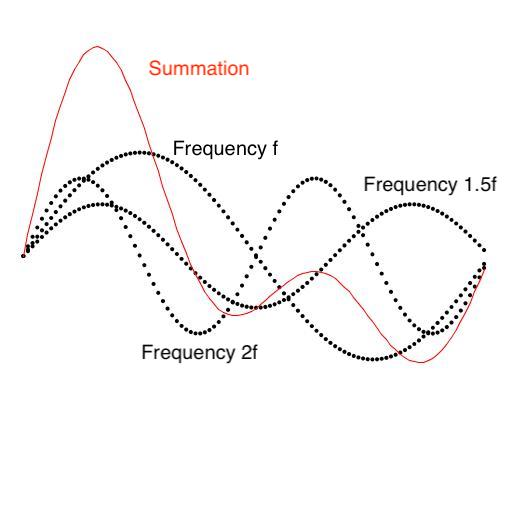
\includegraphics[width=0.8\textwidth]{31/instr.jpeg}
    \end{center}
}{%
\only<1>{%
\begin{itemize}
    \item Sine waves are plotted above at frequencies $f$, $2f$, and $1.5f$.
    \item If those frequencies sound at the same time, the red wave shows the resulting signal that reaches our ears:  the summation of the three black waves.
\end{itemize}
}%
\only<2>{%
Fourier analysis expresses the red wave in terms of the black waves, whose summation equals or approximates the red wave.  In this example, each black wave has the same weight.  In the more general setting, Fourier analysis determines the weight of each sine wave that contributes to the red wave.
}%
}%
%
\Vskip{-1.5em}\begin{itemize}
    \item Remarkably, our brain performs Fourier analysis on the red signal, informing us that we hear a pitch, an octave above that pitch, and the ``fifth'' in between the other two pitches.
    \item This is how our brain can distinguish the sounds of trombones, clarinets, violins, and pipe organs.
   
\end{itemize}%

\end{frame}

\begin{frame}{Some videos worth watching}{From Grant Sanderson's \href{https://www.3blue1brown.com/}{3blue1brown}, these nicely illustrate the Fourier transform}

\begin{itemize}
    \item \href{https://www.youtube.com/watch?v=spUNpyF58BY}{Visual introduction to Fourier}
    \item \href{https://www.youtube.com/watch?v=r6sGWTCMz2k}{How Fourier works}
    \item \href{https://www.youtube.com/watch?v=MBnnXbOM5S4}{Uncertainty principle, regarding Fourier transforms}
\end{itemize}
    
\end{frame}


\begin{frame}{Quantum Fourier}{As compared with Phase Estimation}
\TwoColumns{%
Phase estimation considers the state
\[
\QState{} = \RootTwoN{n}\SumPH{y}{n} \ExpPhase{2\pi \frac{x}{2^n} y} \ket{y}
\]
and computes \ket{x}.
}{%
Quantum Fourier takes a basis state \ket{x} and generates the state
\begin{align*}
\QState{} &= \RootTwoN{n}\SumPH{y}{n} \ExpPhase{2\pi \frac{x}{2^n} y} \ket{y} \\
   &= \RootTwoN{n}\SumPH{y}{n} \ExpPhase{2\pi \frac{y}{2^n} x} \ket{y} 
\end{align*}
}%
\BigSkip{}
So, one operation is the reverse of the other.  We will see this clearly when discussing the circuit for QFT.
\end{frame}
{%
\def\QT#1#2{\ExpPhase{2\pi \alert<#2>{\frac{#1}{2^n} x}} \ket{#1}}
\def\QTO#1#2{\visible<#2->{\ExpPhase{\frac{2\pi}{2^n}\, \alert<#2>{#1\cdot x}}\ket{#1}}}
\def\Space{\hbox to 4em{\hss}}
\begin{frame}{QFT}{The summation}
\Vskip{-3em}\[ \QFT(\ket{x}) = \RootTwoN{n}\SumPH{y}{n} \ExpPhase{2\pi \frac{y}{2^n} x} \ket{y}\]
\Vskip{-4em}\TwoColumns{%
\begin{align*}
       &= \RootTwoN{n}   \left[\  \QT{0}{2} \right. \\
         &\Space{}+ \QT{1}{3} \\
         &\Space{}+ \QT{2}{4} \\
         &\Space{}+ \RVDots{} \\
         &\Space{}+ \left. \QT{2^{n-1}}{5} \ \right] 
\end{align*}
}{%
\begin{align*}
       &= \RootTwoN{n}   \left[\  \QTO{0}{2} \right. \\
         &\Space{}+ \QTO{1}{3} \\
         &\Space{}+ \QTO{2}{4} \\
         &\Space{}+ \RVDots{} \\
         &\Space{}+ \left. \QTO{2^{n-1}}{5} \ \right] 
\end{align*}
}%
\BigSkip{}
The $\cdot$ is simple multiplication, and $x$ takes on a value in $[0,1, \ldots, 2^{n}-1]$.
\end{frame}
}

\begin{frame}{Example}{For $n=2$ qubits, so $x\in [0, 1, 2, 3]$}
\end{frame}